\chapter{Overview on Network Emulation}
\label{chapter2}
Before utilizing the EMANE tool and presenting several situations the tool can be used for, we must first be understood why EMANE was selected and why network emulation is used over simulation or hardware testbeds in this thesis.
After justifying the choices behind selecting EMANE, an in-depth tutorial on the installation, configuration, and operation of the tool is presented.
Finally, a brief overview of mobile ad-hoc network (MANET) routing protocols is presented.
These protocols are essential to understand as they are commonly used in EMANE to create routes between nodes.\par

\section{Testing Communication Networks} % General information on network emulation and simulation and hardware testbeds
There are typically three ways new network architectures, technologies, and protocols are developed and tested. These are network simulation, network emulation, and hardware testbeds~\cite{simulation_emulation}.
As expected each of the three methods has pros and cons.\par
    % Network Hardware
        % Expensive
        % Time consuming to deploy
        % Errors can be sporadic
Hardware testbeds are the most accurate since they encompass the devices expected to be used in the network once development and testing is done.
Hardware, however, is expensive to purchase, time-consuming to deploy, and often difficult to troubleshoot if errors do not consistently appear~\cite{nsclick}.
This makes hardware testing not accessible to users that have a low budget.\par
    % Network Simulation
        % Mimic the behavior of a network
        % Uses mathematical models
        % Can run faster than real time
Network simulation is one solution to testing that appears to solve many of the issues with testing on hardware.
Several free and open-source network simulators like ns-3~\cite{ns3} or OMNeT++~\cite{omnet++} are commonly use and provide a solution to the high costs of hardware.
Like most network simulators, these simulators operate on the concept that the behavior of a network and its components can be modeled via statistical and mathematical models.
Creating models for network behavior allows simulators to run faster than real time since the models do not need to wait for effects to actually happen.
The caveat to this, however, is that simulation models need to be highly accurate when developed or else results from the simulation will not match expected hardware behavior.
Researchers creating new simulation models must ensure the models are validated against the expected hardware behavior to ensure the accuracy of the models, before they are can be used in testing~\cite{omnet_manager}.
Simulation also has the benefit of being highly repeatable since the behavior of the network can be more tightly controlled and any random processes can be set up to repeat previous random outputs~\cite{simulation_emulation}.\par
    % Network Emulation
        % Operates on real network data
        % Allows integration with hardware
        % Potentially more overhead
Network emulation exists somewhere between testing on hardware and testing inside a simulation.
These emulators are still software that gets used to mirror the behavior of a testbed like simulators, but emulators operate on real network data instead of modeling the behavior of a network.
Because emulation testbeds operate on actual network traffic, they also have the ability to interface with hardware allowing hardware testing without building a full hardware network.
This characteristic of operating on real network traffic also has the downside of introducing more computation overhead.
The system emulating the network needs to not only manage all the test traffic, but also manage all the effects and permutations that are imparted on the traffic.\par

% Table summarizing differences between three methods
\begin{table}[!ht]
	\caption{Pros and Cons of Different Types of Network Testing}
	\begin{adjustbox}{width=\textwidth, center=\textwidth}
		\begin{tabular}{|l|l|l|}
			\hline
			Testbed Type & Pros                                                                                                                                                                       & Cons                                                                                                                                                                  \\
			\toprule
			Hardware     & \begin{tabular}{@{\labelitemi\hspace{\dimexpr\labelsep+0.5\tabcolsep}}l@{}}Highly accurate\\Does not require modification of networking software\end{tabular}                                 & \begin{tabular}{@{\labelitemi\hspace{\dimexpr\labelsep+0.5\tabcolsep}}l@{}}Expensive to build\\Time consuming to deploy and configure\\Errors can be sporadic\end{tabular}               \\
			\hline
			Simulation   & \begin{tabular}{@{\labelitemi\hspace{\dimexpr\labelsep+0.5\tabcolsep}}l@{}}Free tools available\\Can run faster than real time\\Easy to reconfigure and modify\end{tabular}                   & \begin{tabular}{@{\labelitemi\hspace{\dimexpr\labelsep+0.5\tabcolsep}}l@{}}Models must be designed to be highly accurate\\Software must be translated to a simulation model\end{tabular} \\
			\hline
			Emulation    & \begin{tabular}{@{\labelitemi\hspace{\dimexpr\labelsep+0.5\tabcolsep}}l@{}}Free tools available\\Can run native implementations of network software\\Can interface with hardware\end{tabular} & \begin{tabular}{@{\labelitemi\hspace{\dimexpr\labelsep+0.5\tabcolsep}}l@{}}Must run in real time\\Requires higher computational overhead\end{tabular}                                    \\
			\hline
		\end{tabular}
	\end{adjustbox}
	\label{simtable}
\end{table}

Table~\ref{simtable} summarizes the pros and cons of different testing environments.

\section{Evaluation of Network Testing Tools} % Why EMANE was selected over other tools
There are several network simulation and emulation tools that were considered for use in this thesis during initial research.
These programs all provide functionality that would achieve the goals of performing inexpensive and less time-consuming network testing, but were eventually decided against in favor of EMANE.
This section will highlight a few of these tools and explain the reasoning behind why they were not selected, before finishing by introducing EMANE and the driving reasons for its selection.\par

% ns-2 and ns-3
One of the most common tools, ns-3, is a discrete event-based network simulation tool that is commonly used for simulation of TCP/IP networks~\cite{ns3}.
It is the successor to the ns-2 tool~\cite{ns2}, with the two major differences being the method that simulation scripts are written and how these scripts are executed in the simulator.
In ns-3 the core simulator as well as experiment scripts are written in C++ and ns-3 provides bindings for Python so simpler scripts can also be written in Python.
This is much simpler than ns-2 which required the use of Tcl scripts to create experiments~\cite{ns2_ns3}.
The migration from ns-2's method of programming to ns-3's makes the tool easier to use, but it does still require an amount of programming knowledge to understand how utilize the library of models provided.
Being one of the most commonly used tools, ns-3's library of simulation modules have been extensively validated, but these modules typically focus on the network layer and above.
ns-3 does have the ability to be used as an emulator, however the motivation emulation mode in ns-3 was primarily driven by the ability to use ns-3 with hardware~\cite{ns3_orbit}.
Since we would like to avoid hardware wireless equipment, this option for ns-3 is not valuable for the research present in this paper.
The wide-scale use and extensive support of ns-3 made the tool a promising candidate, but it was decided against due to the abstractions made at the physical layer.\par

% OMNeT++
OMNeT++ is another discrete event simulator written in C++, like ns-3, however it is not specifically designed as a communications network simulator~\cite{omnet++}.
Despite not being designed as a communications network simulator, the ability to create plugins for the tool has led to many researchers creating models of communication networks that can be used for simulation.
The issue with this collection of plugins is that many users have found them to be highly incompatible with each other. This is likely due to the isolated nature many of the models were developed under~\cite{tool_survey}
One of the advantages of OMNeT++ is that is supports a graphical user interface, that allows for easier building of and interaction with network testbeds.
Figure~\ref{omnet_gui} shows an example of this GUI, which is based off of the Eclipse IDE.\par

\begin{figure}[!ht]
    \centering
    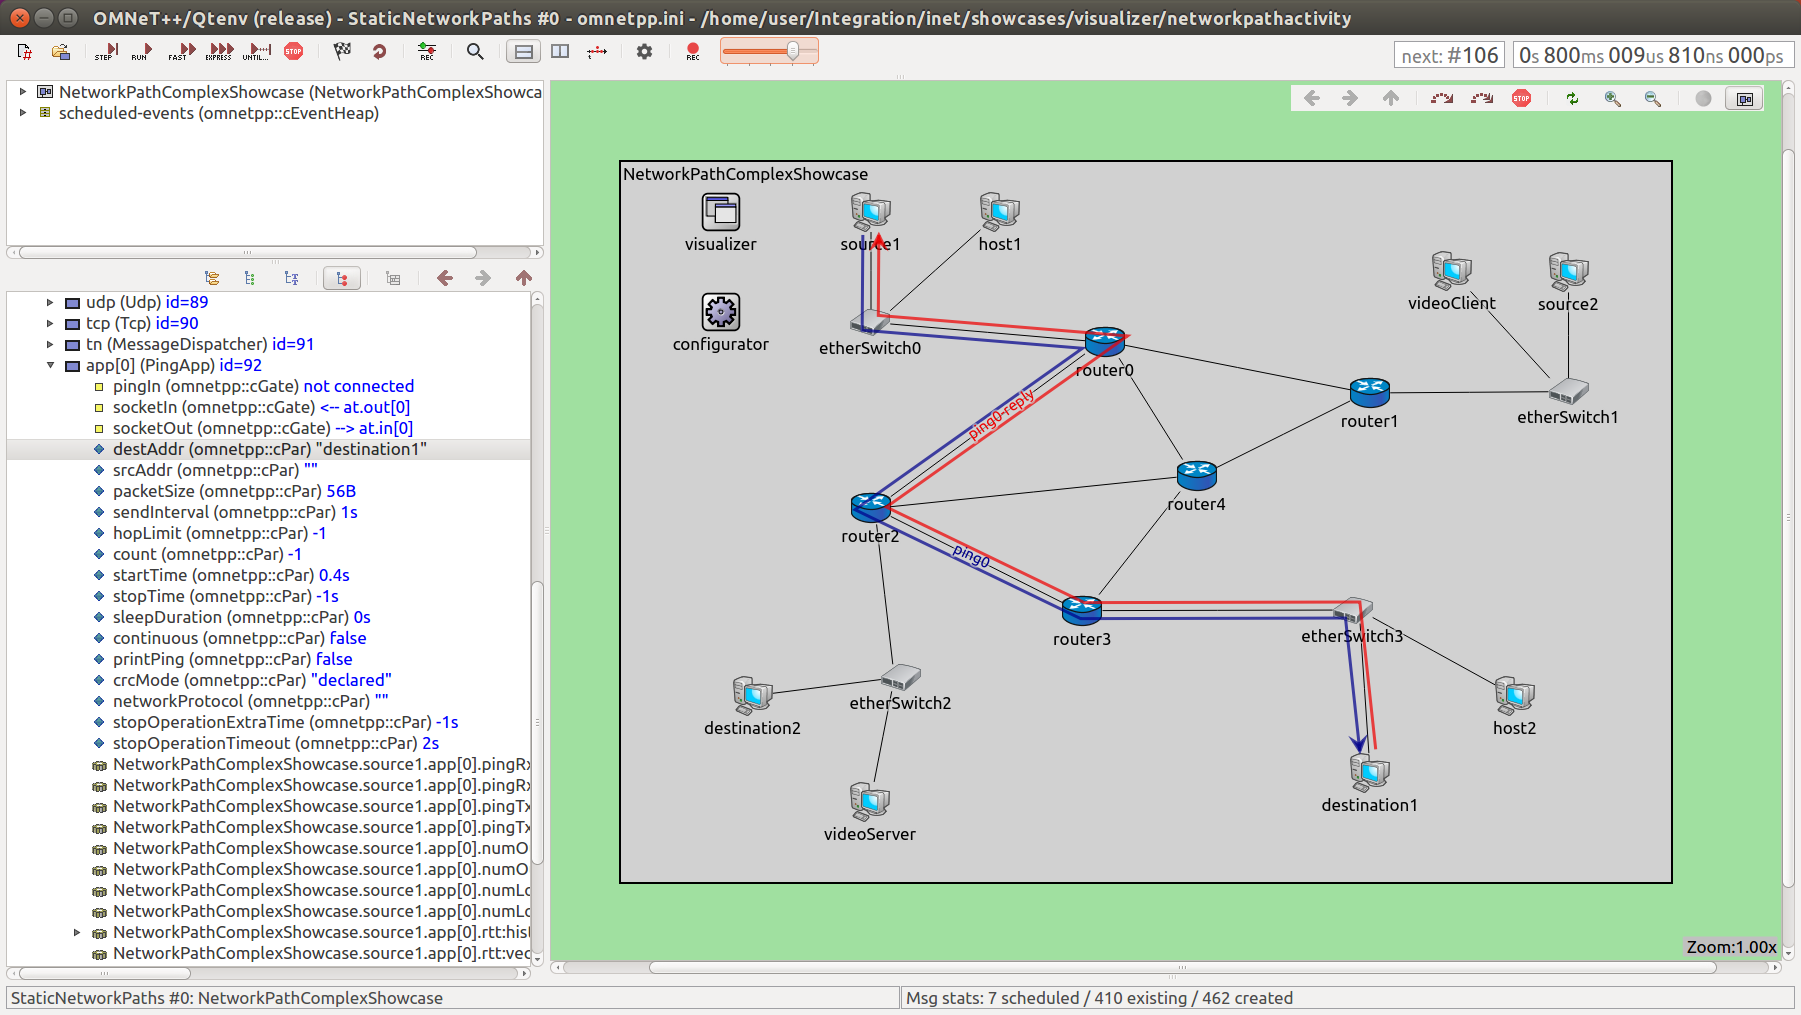
\includegraphics[width=\textwidth,keepaspectratio]{Images/Chpt2/omnet_gui.png}
    \caption{An example of the OMNeT++ Simulator GUI.}
    \label{omnet_gui}
\end{figure}

% CORE
The Common Open Research Emulator (CORE) is an emulation tool focused on emulation of layers three (network layer) and above in the OSI stack \cite{core}.
Of all the tools presented so far, CORE is one of the easiest to use.
Similar to OMNeT++, CORE provides the user with a GUI that takes the form of a blank canvas where users can drag and drop preconfigured nodes such as routers and servers.
Figure~\ref{core_gui} is a basic example of what a typical CORE session looks like.
CORE also gives users the ability to create virtual nodes via a Python framework, that is useful for more complex scenarios.
Without any modification, CORE emulates the network layer and above perfectly, as each virtual node is running the actual, unmodified software that would be running on hardware \cite{emane_core}.
Where CORE runs into issues is when wireless channels are introduced.
By default, CORE operates on the concept that nodes that are close enough to communicate they have a connection, and if they are far enough by a certain distance, they can not communicate.
This simplification is not acceptable for a majority of testing that requires accurate wireless communication modeling, and so to solve this issue EMANE was integrated into CORE so that all physical and data link layer emulation happened through EMANE \cite{emane_core}.
Figure~\ref{core_emane} shows the configuration menu for EMANE, within CORE.
With this pairing CORE and EMANE become a very valuable tool, however in this thesis CORE is not used, independently or alongside EMANE.
The main reasoning for this is because a majority of the protocols being used at the network layer or higher, are not present in CORE and computational complexity can be saved by running them in EMANE directly, without CORE.\par

\begin{figure}[!ht]
    \centering
    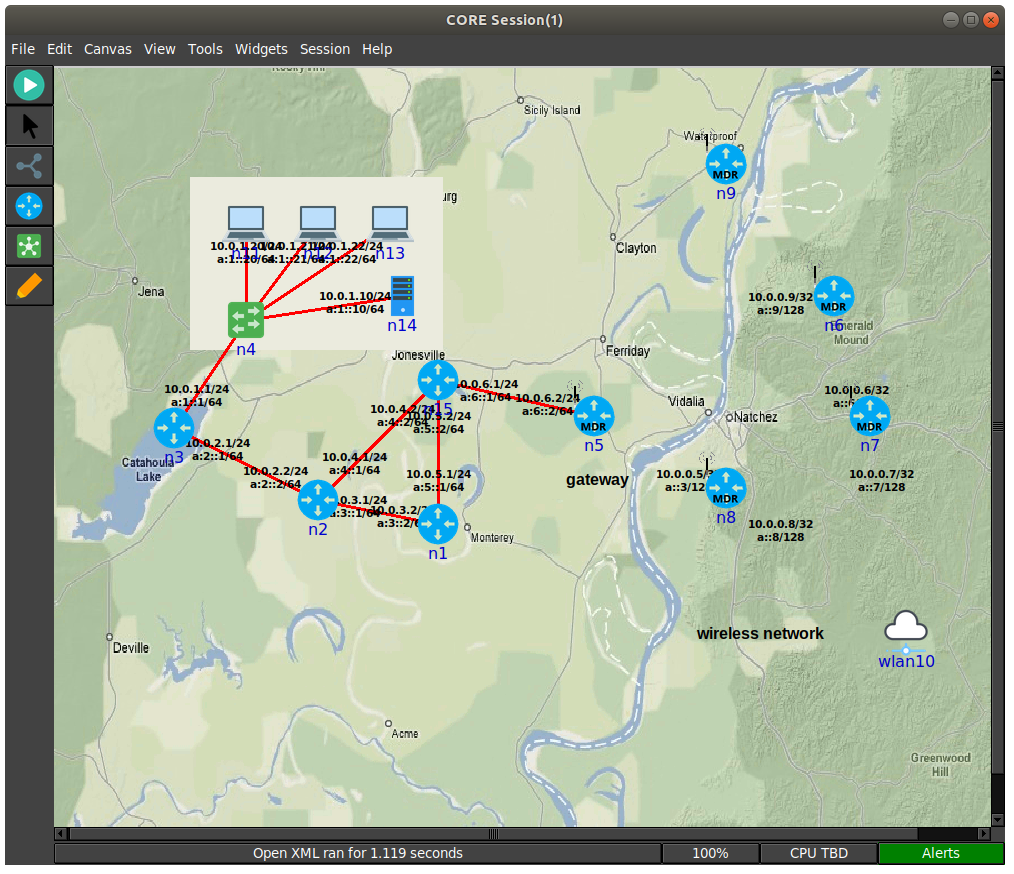
\includegraphics[width=\textwidth,keepaspectratio]{Images/Chpt2/core_gui.png}
    \caption{An example of the CORE Emulator GUI.}
    \label{core_gui}
\end{figure}

\begin{figure}[!ht]
    \centering
    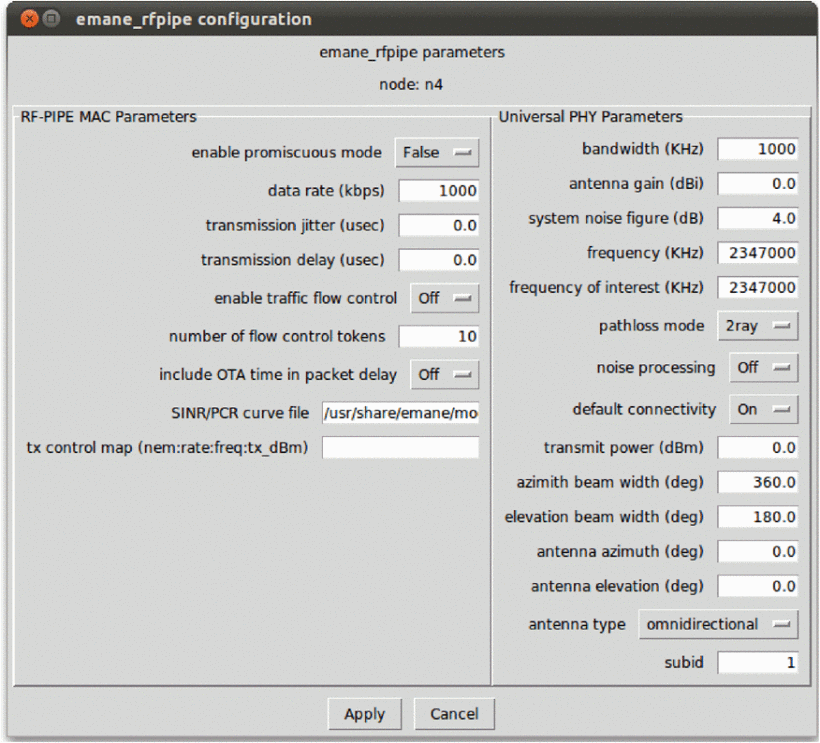
\includegraphics[width=\textwidth,keepaspectratio]{Images/Chpt2/core_emane.png}
    \caption{The configuration menu for EMANE, within CORE. From~\cite{emane_core}.}
    \label{core_emane}
\end{figure}

% EMANE
EMANE is a network emulation tool originally developed by the Naval Research Lab and currently maintained by AdjacentLink LLC~\cite{emane_nrl}.
The tool is a discrete event-driven emulator programmed in C++ and Python, and is configured by the user primarily through XML files and Bash scripts.
The software was developed with the intention of creating a platform that could emulate the physical and data link layers of the OSI network model with high accuracy, avoiding many of the abstractions made by other tools.
EMANE consists of several subsystems and components required to create a fully functional testbed, and this complexity can lead to an initial steep learning curve with the tool.
The tool is open-source, however, the online community around EMANE is rather small and most of the discussion and troubleshooting surrounding the tool is only found on EMANE's GitHub issues page, not helping with the complexity issue.
Despite all this, once the user forms a core understanding of the tools and systems within the software, the tool can be used to effectively and quickly create model wireless networks.
EMANE's ability to be configured through XML makes deployment of networks very rapid, and because the included models are pluggable, these configuration files can be reused completely independently of the topology of the nodes in the network.
For these reasons and the reasons highlighted previously regarding other testing tools, EMANE was selected as the tool of choice for this thesis and the next section is dedicated to understanding how to both install the tool, and how all the pieces work together.\par

Table~\ref{tooltable} highlights the main advantages and disadvantages of each of these tools.

\begin{table}[!ht]
	\caption{Overview of Advantages and Disadvantages of Different Networking Testing Tools}
	\begin{adjustbox}{width=\textwidth, center=\textwidth}
        \begin{tabular}{|l|c|c|} 
        \hline
        \multicolumn{1}{|c|}{Tool} & Advantages & Disadvantages \\ 
        \toprule
        ns-3 & \begin{tabular}[c]{@{}c@{}}Open-source\\Extensive protocol library\\Widely used and validated\end{tabular} & \begin{tabular}[c]{@{}c@{}}Abstracts the PHY and MAC layers\\Limited control of individual nodes\\Simple wireless propagation models\end{tabular} \\ 
        \hline
        OMNeT++ & \begin{tabular}[c]{@{}c@{}}GUI-based\\Large library of models\end{tabular} & \begin{tabular}[c]{@{}c@{}}Not purpose built for network simulation\\Provided models are often not compatible\end{tabular} \\ 
        \hline
        CORE & \begin{tabular}[c]{@{}c@{}}Open-source\\GUI-based\\Simple models do not require programming knowledge\end{tabular} & \begin{tabular}[c]{@{}c@{}}Only emulates the network layer and above\\Limited network protocols available by default\end{tabular} \\ 
        \hline
        EMANE & \begin{tabular}[c]{@{}c@{}}Open-source\\Purpose built to emulate PHY and MAC layer\\Can use any implementation of network software\end{tabular} & \begin{tabular}[c]{@{}c@{}}Small online community\\Initial steep learning curve\\Requires extensive computing resources for large-scale networks\end{tabular} \\
        \hline
        \end{tabular}
	\end{adjustbox}
	\label{tooltable}
\end{table}

\section{Using EMANE}
Having selected EMANE for use in this thesis, we must now understand how to install, configure, and operate the tool.
This section will begin by detailing the installation of EMANE, 
EMANE can be installed and used in a few distinct ways.
The primary two methods are installation via the bundle of pre-built binaries provided by AdjacentLink or building all the required programs from source.
Compiling the software from source is typically only necessary when making extensions to the tool, such as adding custom modules.
Since only the default included modules are used, the precompiled bundle is sufficient for the work completed in this thesis.
The installation instructions for EMANE can be found in~\cite{emane_tutorial}, but it should be noted that these instructions are sometimes out of date.
The full EMANE GitHub repository~\cite{emane_git} may also provide guidance that is more up to date.
EMANE version 1.3.3 was the primary version of the tool used in this work, and supports the Rocky 8, Fedora 37, and Ubuntu 20.04 Linux distributions.\par
    % Basic installation instructions
        % Download binary packages
        % Install pre-complied bundle
        % Verify programs are installed
        % Optionally: Install extra software
These instructions assume a fresh installation of Ubuntu 20.04.04 is being used and that is system is up-to-date with the latest software.
If a different supported distribution of Linux is used, the steps will be similar, however the commands will differ. Refer to~\cite{emane_tutorial,emane_git} for further details.
See Appendix~\ref{appendixa} for a list of the specific commands run to complete the entire installation process.
\begin{enumerate}
    \item The first step is downloading the precompiled binaries. As seen in Figure~\ref{wget_emane}, the \textit{wget} utility is used to download the compressed file, but any method for retrieving this file can be used. This compressed file should be extracted before the next step.
    \item To install the downloaded binaries, the \textit{dpkg} application is used. Errors will be reported upon installation, as not all the dependencies are installed. This will be fixed after the initial installation via \textit{apt}. Figure~\ref{install_emane} shows the initial installation finishing with errors, and the command used to fix these errors.
    \item Lastly, we can verify that EMANE was installed correctly by having the program output its version. Figure~\ref{check_emane} shows that EMANE version 1.3.3 was successfully installed.
    \item Once installation of EMANE has been verified, additional support software (like testing tools and routing protocols) can be installed to use with EMANE. Appendix~\ref{appendixa} shows some examples of installing certain tools.
\end{enumerate}

\begin{figure}[!ht]
    \centering
    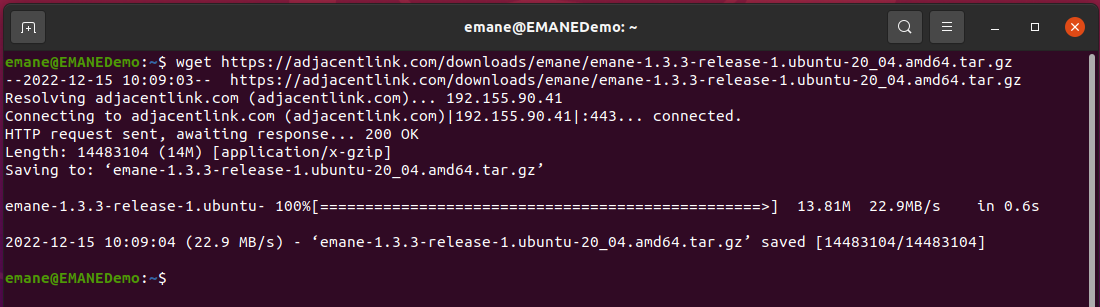
\includegraphics[width=\textwidth,keepaspectratio]{Images/Chpt2/wgetEMANE.png}
    \caption{Downloading the precompiled EMANE binaries using the \textit{wget} command.}
    \label{wget_emane}
\end{figure}

\begin{figure}[!ht]
    \centering
    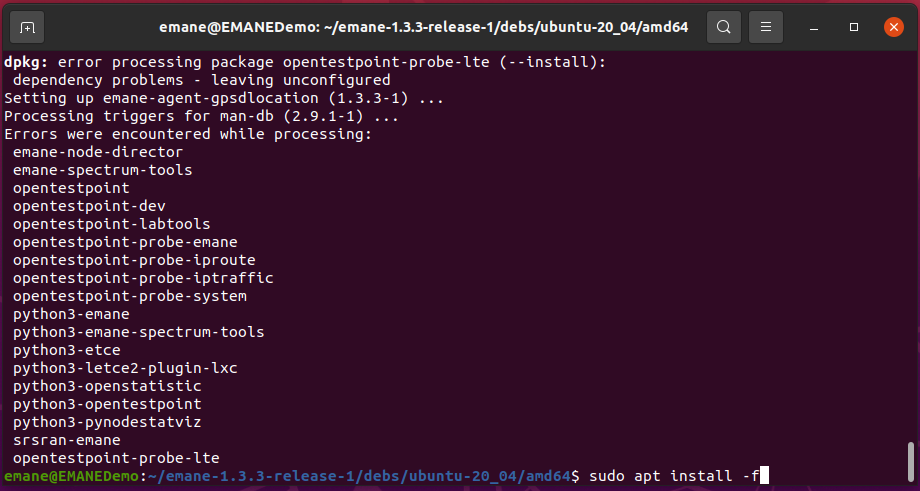
\includegraphics[width=\textwidth,keepaspectratio]{Images/Chpt2/dpkgEMANE.png}
    \caption{Installing the EMANE program \textit{dpkg} command.}
    \label{install_emane}
\end{figure}

\begin{figure}[!ht]
    \centering
    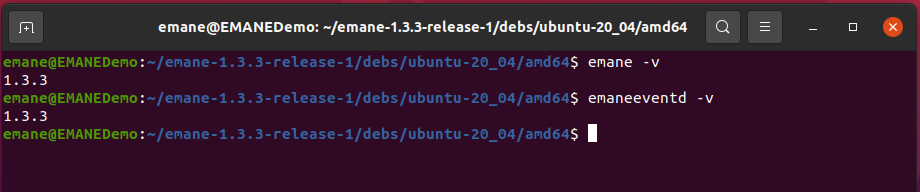
\includegraphics[width=\textwidth,keepaspectratio]{Images/Chpt2/versionEMANE.png}
    \caption{Verifying EMANE installed correctly by displaying the version number.}
    \label{check_emane}
\end{figure}

    % Basic architecture overview
    % NEMs
        % Each NEM should exist on its own platform server inside its own LXC
            % EMANE recommends not putting multiple NEMs on one platform server for performance reasons
            % Each platform server (running instance of EMANE) needs to have network stack isolation (accomplished via LXCs, but other methods exist)
        % Each NEM has 3 layers, PHY layer, Radio layer, and transport layer
        % Each NEM also interfaces with the event engine to ensure proper configuration and processing
Now that EMANE is installed, it is important to understand the major systems that work together to enable network emulation.
The main structure in EMANE that everything operates around is known as the Network Emulation Module (NEM).
Each NEM can be thought of as a single network node, similar to a singular radio.
As each NEM is an independent network node, every NEM created requires network stack isolation within the kernel of the host system.
All the traffic flowing through the emulation testbed consists of real IP packets and are therefore treated like regular network traffic by the kernel.
If the network stacks were not isolated, packets would not route through the emulator and would instead just be switched between processes in the kernel, bypassing all wireless channel effects.\par
There are several methods than can be used to create network stack isolation.
Full virtual machines could be used, but these are very computationally inefficient and would not allow the emulated testbed to maintain a large amount of nodes.
Additionally, nodes in EMANE do not need the full isolation provided by virtual machines, and it is even beneficial if the file system could be shared.
To solve this problem, containers are used as the primary method of isolation.
\cite{core_containers} examines several types of virtualization that can be used for isolation nodes in CORE, but the same concepts apply to EMANE.
Between FreeBSD jails, Linux OpenVZ containers, and Linux namespaces containers, the namespaces containers are found to be the most efficient.
For most examples of EMANE and all the testbeds created in this thesis, Linux Containers (LXCs) are used.
These are lightweight containers that are built on top of Linux namespaces and allow for the sharing of files and other resources, while keeping processes and the network stack isolated.\par

Figure~\ref{emane_diagram} shows what a typical EMANE emulation node will look like, with one of these structures existing per LXC.
In this diagram, the NEM is visible, with all of its surrounding subsystems and connections.
The blue boxes within the NEM are the emulation models that are responsible for imparting wireless channel effects on packets moving upstream and downstream through the emulator.
The green boxes represent the transport boundary. This is the edge of the emulation node where packets leave the emulator and return to normal application space.
The orange box represents the event service that is responsible for changing the state and settings of the emulator during runtime in order to create effects in the network.
These three systems are the major subsystems that make up EMANE and allow it to create highly dynamic networks, used to test a variety of use cases and will be examined in depth in the next three subsections.

\begin{figure}[!ht]
    \centering
    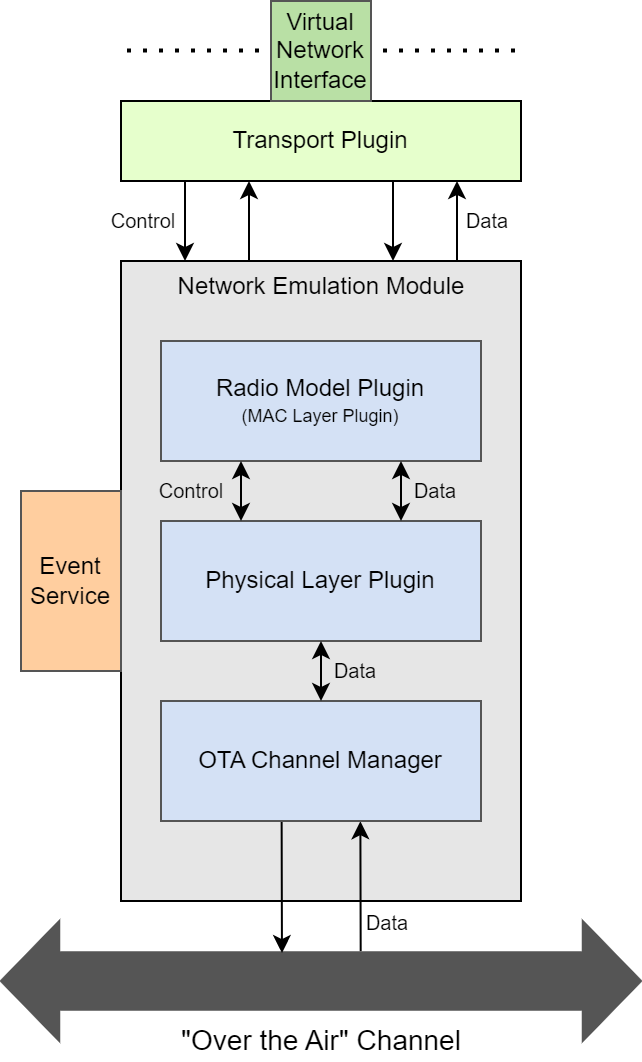
\includegraphics[width=0.5\textwidth,keepaspectratio]{Images/Chpt2/emane_diagram.png}
    \caption{An overview of an individual EMANE emulated network node.}
    \label{emane_diagram}
\end{figure}

\subsection{Emulation Model Processing}
    % Emulation Model Processing
The emulation model processing is the system primarily responsible for modifying packets traveling through the NEM to mimic the behavior of a wireless signal.
This system of EMANE consists of two main parts, the Physical Layer Plugin and the Radio Model Plugin, both of which can be seen in blue in Figure~\ref{emane_diagram}.
As the names of the plugins imply, the Physical Layer plugin is responsible for imparting the effects of the physical layer, and the Radio model plugin is responsible for the MAC Layer.
The Over the Air Channel Manager is primarily just responsible for pulling packets addressed to the NEM, off of the shared bus, and putting packets ready to be transmitted onto the shared channel.
This shared OTA channel simply takes the form of a virtual interface bridge that all the NEMs are attached to, creating a bus topology.
The NEMs use a multicast scheme to listen for packets as other control channels also use this interface bridge to communicate.
It is the main backbone of the emulation that connects all the individual network nodes, both for control messages, but also data payloads.\par
    % Shared PHY model
        % Pathloss, fading, noise, pulling packets of OTA channel, power calculations
As previously mentioned, the shared PHY plugin is responsible for the effects of the physical layer.
It is possible to create a custom Physical Layer model, but is usually not necessary and is the only PHY model included in EMANE.
This model is responsible for attributes like pathloss and signal propagation, fading, noise modeling, the antenna profile.\par
The first parameter to be set is the propagation model.
This model is responsible for calculating the expected pathloss between two nodes, and has three options.
The first two options are \textit{freespace} and \textit{2ray}.
These use location data contained within the node and the freespace or 2-ray flat earth model to calculate the pathloss of a channel.
The third option is called \textit{precomputed} and is used when the pathloss is to be calculated external to the emulator.
This is useful if a more complex model is to be used, or a different tool is being used to model signal propagation.\par
The second configuration step is related to the power characteristics of the node and its virtual antenna.
Transmit power can be set, and serves the same purpose it would on a hardware radio.
The antenna gains can be set as a static value, or a more complex profile that contains a list of antenna pattern entries.
The following is an example of the contents of an antenna profile file from the CORE/EMANE documentation~\cite{core}:
\begin{center}
\begin{minipage}{\textwidth}
    \begin{minted}[fontsize=\small, breaklines]{xml}
    <!-- 30degree sector antenna pattern with main beam at +6dB and gain decreasing by 3dB every 5 degrees in elevation or bearing.-->
    <antennaprofile>
      <antennapattern>
        <elevation min='-90' max='-16'>
          <bearing min='0' max='359'>
            <gain value='-200'/>
          </bearing>
        </elevation>
        <elevation min='-15' max='-11'>
          <bearing min='0' max='5'>
            <gain value='0'/>
          </bearing>
    \end{minted}
\end{minipage}
\end{center}\par
The final piece of the PHY model that must be understood is noise modeling.
EMANE models noise by taking the transmission power of any NEM transmitting, and adding it to the noise floor of the receiving node if the receiver's frequency is within the bandwidth of the interfering signal.
This results in all interfering signals being treated as white noise~\cite{emane_phy}.
EMANE provides parameters to set if the noise mode is for all signals within the correct frequency, just signals that are out-of-band, or turning off noise processing completely.
Once all of these factors are set, EMANE can then use the following two equations to determine if a packet can actually be received.
If the received power (\textit{rxPower}) is greater than the receiver's sensitivity (\textit{rxSensitivity}), the packet is received.
\[ rxPower = txPower + txAntennaGain + rxAntennaGain - pathloss \]
\[ rxSensitivity = -174 + noiseFigure + 10log(bandwidth) \]
Figure~\ref{emane_phy} shows what a general Physical Layer Plugin configuration file will look like.\par

\begin{figure}[!ht]
    \centering
    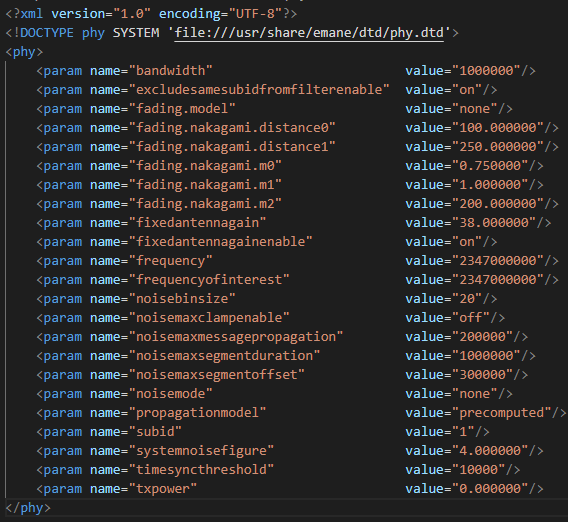
\includegraphics[width=0.8\textwidth,keepaspectratio]{Images/Chpt2/emane_phy.png}
    \caption{A generic configuration file for an EMANE PHY Plugin}
    \label{emane_phy}
\end{figure}

    % Radio model
        % Data bandwidth, delay, more advance medium access control schemes, SINR packet drop probabilities
The second piece of the emulation model processing layer of EMANE is the Radio Model plugins.
Unlike the PHY plugin which is shared for all NEMs, the Radio plugin is different depending on the type of waveform emulation desired.
EMANE ships with four Radio plugins:
\begin{itemize}
    \item rfPipe - A generic wireless channel that does not do channel access functions
    \item IEEE802.11abg - A model specifically for 2.4GHz Wi-Fi waveforms
    \item TDMA - A generic time division multiple access scheme
    \item Bypass - A model specifically for testing that passes traffic along to the next layer unchanged
\end{itemize}
Other plugins can be created by extending the emulator, and a plugin designed for LTE and 5G is currently under development in collaboration with the srsRAN project.\par
These four plugins all operate differently, but for the purposes of this thesis only the rfPipe model will be used.
The goal of the rfPipe model is to create a simple model that handles data rate, delay, jitter, and probability of packet loss due to signal to interference and noise ratio (SINR).
The data rate, delay, and jitter are all simple parameters that get set and are implemented by holding packets at the radio model layer long enough to achieve the set values.
The Packet Completion Rate (PCR) utilizes the signal, interference, and noise power levels calculated by the Physical Layer model to find the SINR value, and compares that to a lookup table.
The portion of the table and corresponding curves, as seen in Figure~\ref{emane_pcr}, are used to come up with a probability value that is used to decided if the packet should be lost or otherwise corrupted due to noise.

\begin{figure}[!ht]
    \centering
    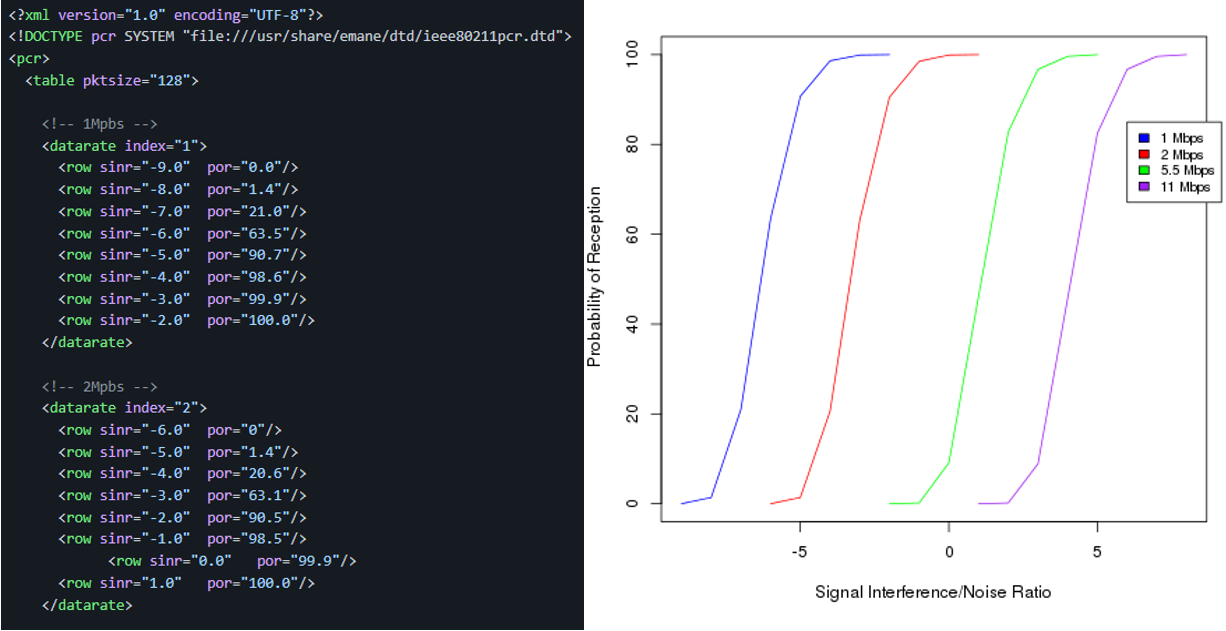
\includegraphics[width=\textwidth,keepaspectratio]{Images/Chpt2/emane_pcr.png}
    \caption{The packet complete rate (PCR) table and corresponding curve.}
    \label{emane_pcr}
\end{figure}

One of the essential pieces of the emulation processing system is ensuring the models used are accurate to hardware, to ensure results used from the emulator are accurate.
While several studies use the rfPipe model \cite{rfPipe1, rfPipe2, rfPipe3}, very little literature could be found validating the models included within EMANE.
The rfPipe model is generic enough that there are no modulation schemes or other access functions that need to be validated, but the implementation of the behavior must still be checked.
Similarly, the calculations performed at the Physical Layer are fairly simple, but must also be validated.
A validation like the one found for the TDMA model \cite{emane_tdma}, should be performed for all models presently in EMANE, as well as for any custom models created.
For the purposes of this thesis, EMANE is being used to model parameters like throughput and latency which can be easily compared to hardware equivalent testbeds.
Chapter 3 will examine this to make comparisons between the two, however, if EMANE is to be used in more advanced testbeds with highly complex models, validation is essential.

\subsection{Transport Boundary Processing}
    % Transport Boundary Processing
The second system required to operate EMANE is the transport boundary.
The transport boundary is represented in Figure~\ref{emane_diagram} by the green boxes, and is responsible for handing packets entering and exiting the emulator.
Since EMANE is capable on operating on actual TCP/IP packets, one of the main roles of the transport boundary is to translate TCP/IP packets entering the emulator into something EMANE can operate on, and translate EMANE's packet back into TCP/IP packets.
There are two types of transports that can be used with EMANE, raw transports and virtual transports.\par
    % Raw transport
        % Use physical network device as edge of emulation
        % Allows for "black-box" style testing
        % Can be used to interface physical networking hardware with EMANE
Raw transports are used for enabling the hardware in the loop functionality of EMANE.
When a raw transport plugin is initialized, it is connected to a hardware network interface present on the emulation host machine.
This breaks the convention of having EMANE nodes exist within LXCs, but if only one EMANE node is present on the host the node can run external to a virtualized environment.
If multiple nodes exist, a pair of virtual network interfaces can be created and bridged to the hardware interface to create a tunnel from inside the LXC to the hardware interface on the host.
This method is used in Chapters 3 and 4 and will be outlined in more detail there.
Figure~\ref{emane_raw_transport} shows an example of the layout of the network interface on the host and the EMANE instance.

\begin{figure}[!ht]
    \centering
    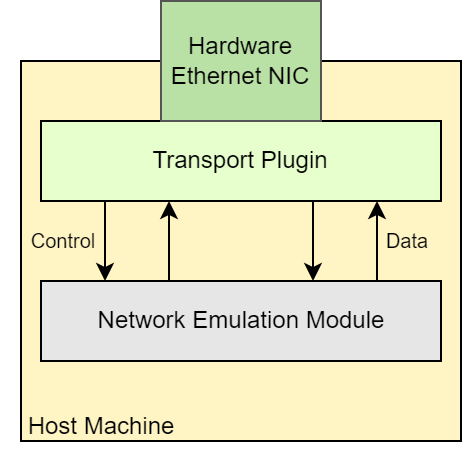
\includegraphics[width=0.5\textwidth,keepaspectratio]{Images/Chpt2/RawTransport.png}
    \caption{An example EMANE topology using the raw transport plugin.}
    \label{emane_raw_transport}
\end{figure}

    % Virtual transport
        % Uses virtual kernel interfaces as edge of emulation
        % Internal transports
            % For NEMS on the same platform server, packets are not even sent through kernel devices, just shared with each other in memory
        % External transports
            % NEMs on different platforms servers must share data through the kernel (since they will have network stack isolation)
The second type of transport are virtual transport plugins.
These are more commonly used as they are the plugins that carry from the emulator instance to application space via a virtual network interface.
When EMANE is started on an LXC using a virtual transport, the LXC is created with a pair of virtual interfaces.
One of the interfaces is internal to the LXC and is used as the endpoint for EMANE, the other is external to the LXC and is bridged together with all the other nodes to allow traffic to pass.
Figure~\ref{emane_virtual_transport} shows an example of the layout of the virtual network interfaces bridged together between EMANE instances, internal on the host machine.

\begin{figure}[!ht]
    \centering
    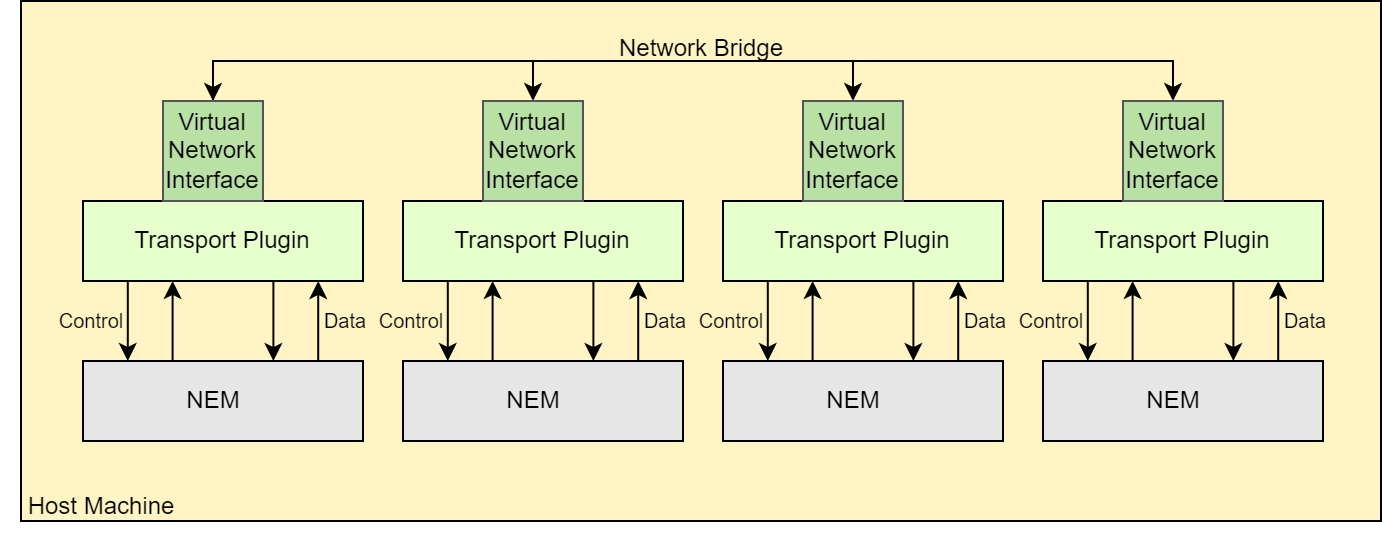
\includegraphics[width=\textwidth,keepaspectratio]{Images/Chpt2/VirtualTransport.png}
    \caption{An example EMANE topology using the virtual transport plugin.}
    \label{emane_virtual_transport}
\end{figure}

\subsection{Event Processing}
    % Event Processing
        % Event channel vs. OTA channel
            % Scripted before runtime
                % EEL file(s)
            % Sent during runtime
                % Python modules
Event processing is the system in EMANE that allows parameters of the simulator to change during runtime.
There are five main event types.
The first type, pathloss, is used when the propagation model is set to \textit{precomputed} and allows an external tool to make pathloss calculations.
The second type, location, is used to move nodes around and primarily influences pathloss values that are calculated internally to the tool when using \textit{freespace} or \textit{2ray} settings.
The location event can take the latitude, longitude, altitude, pitch, yaw, roll, and velocity data for a node.
The third event type is the antenna profile event.
Similar to the antenna profile setting in the Physical Layer plugin, this event can be used to feed antenna data to a node, and change that data during runtime.
The fourth event is used to change the fading model being used.
This event is fairly simple and is used to toggle whether a node uses the Nakagami fading model or no fading model.
The final event is called Comm Effect, and is used to change generic communication parameters of a node, such as the latency, jitter, or probability of packet loss and duplication.\par
    % Scripted before runtime
        % EEL file(s)
    % Sent during runtime
            % Python modules
There are two primary methods that events get generated for distribution to nodes.
The first is using an EEL file.
This file is a specific EMANE file that is taken in at the start of emulation and contains "sentences" that outline event parameters and what time during the simulation they should begin.
Figure~\ref{emane_event} shows an example of an EEL file and the sentences contained within.
The first value is the time the event is scheduled to fire, in this case all of these events fire at the start of emulation.
The second value is the ID of the NEM the event is destined for, and this is followed by the event name and any corresponding parameters.
The other main method for generating events is through Python bindings that allow direct subscription to the event channel for publishing of events.
Events are passed to NEMs via the event channel, but all this channel is, is a different multicast service that the NEMs subscribe to on the same network interface bridge that the over-the-air channel lives on.
By putting both of these channels on the same bridge, the complexity of managing several network devices per NEM is lessened.

\begin{figure}[!ht]
    \centering
    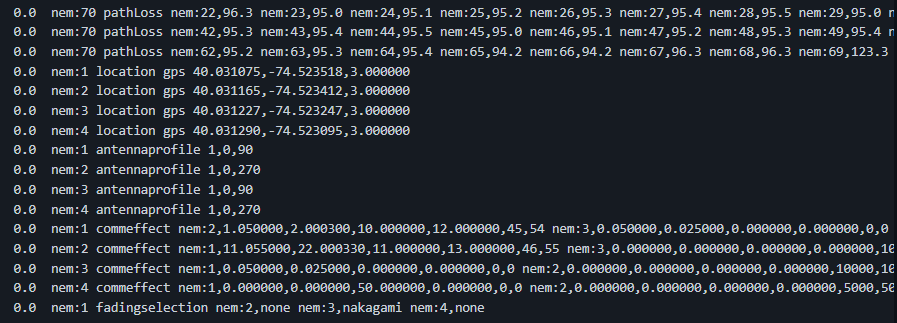
\includegraphics[width=\textwidth,keepaspectratio]{Images/Chpt2/emane_event.png}
    \caption{An example of an EEL file provided to the EMANE event service.}
    \label{emane_event}
\end{figure}

\section{Routing in Mobile Mesh Networks}
    % What is important in routing in a ad-hoc mobile network rather than a traditional network
    % What routing algorithms exist in literature
        % Reactive vs. Proactive
EMANE was designed primarily to work with mobile ad-hoc networks, also known as MANETs, and while emulating other network types is possible, MANET routing protocols work well with EMANE's architecture.
This special classification of network is characterized by its dynamic topology that often rapidly changes due to the mobility of network nodes and the tendency for the wireless links to connect and disconnect~\cite{manet_storm}.
This lack of a fixed topology means that any node that exists in the network must be able to communicate without help from centralized infrastructure or a gateway and therefore must be able to independently make routing decisions. 
Since the topology of a MANET is a mesh, the primary method for traffic traveling through the network is through relaying.
Each node in the mesh acts as a router and upon receiving network traffic, must determine if the traffic is destined for itself, or a different node in the network.
In the second case, the relaying node will use its knowledge of the routing table and network topology to determine which neighbor node the packets must be forwarded to~\cite{manet_survey}.
These types of routing protocols can be separated into two categories, proactive protocols and reactive protocols~\cite{manet_survey}.

\subsection{Proactive Mesh Routing}
        % Requires more overhead
        % Can (keep can, not will) react more quickly to topology changes
        % Periodically send out "discovery" packets to sense link quality/delivery topology info/etc.
The first category of MANET routing protocol is the proactive protocol.
Proactive protocols are similar to traditional routing protocols in the sense that they create and maintain a routing table.
By maintaining a routing table, any transmission that needs to be sent can be done so immediately since the most efficient route is known.
This allows proactive protocols to operate with less latency than reactive MANET routing protocols as they do not need to wait for route discovery at the time of transmission~\cite{manet_performance}.
The caveat to this is that these protocols require much higher control traffic as they must perform periodic link sensing to ensure the routing tables are up-to-date.
In a network where bandwidth is constrained, it is essential to understand this limitation at the time of design as MANETs are often already bandwidth restricted and adding another high usage system could be too much.\par
        % Examples:
            % OLSR
                % Floods network with topology info
            % BATMAN-adv
                % Layer two routing, node only aware of neighbors
                % Depends on neighbors to ensure data is passed along
There are two routing protocols that the maintainers of EMANE often use in examples and tutorials for the tool.
These are the Open Link State Routing (OLSR) protocol~\cite{rfc_olsr} and the Better Approach to Mobile Ad-hoc Networking (B.A.T.M.A.N.) protocol~\cite{batman}. 
These routing protocols are both proactive MANET routing protocols and are two of the more common purpose built proactive protocols found in MANETs.
They both operate on the similar principle of link sensing via a discovery packet (called HELLO packets in OLSR and OGM packets in B.A.T.M.A.N.), but differ in how the best routes are calculated.\par
        % BATMAN general performs better than OLSR in most conditions [cite paper]
When deciding between these two protocols it is found that B.A.T.M.A.N. typically will outperform OLSR~\cite{olsrd_batman}.
This can be attributed to the manner in which OLSR performs link sensing.
When evaluating two paths, the path with the least number of relays is considered the best path in OLSR~\cite{rfc_olsr}.
This concept is feasible in high speed wired networks where queuing and relaying of data is often the slowest portion of a packets journey, but in wireless networks where the quality of the medium can drastically vary, this does not work as well.
B.A.T.M.A.N. attempts to solve this issue by using the concept that the link from which a discovery packet arrives from first, must be the best link to send a packet for it to arrive at the destination in the OGM.
Since the link with the lowest latency and highest throughput is expected to deliver packets the fastest, it can be assumed it is the best link~\cite{batman}.
Since B.A.T.M.A.N. nodes only measure which neighbor has a route to a given destination, and does not share the topology of the entire network graph, the protocol also produces less control traffic, which contributes to it performing better.
Figure~\ref{batman_topology} shows what topology information nodes might have in a network running B.A.T.M.A.N.
Nodes B and C maintain a list that indicates which nodes in the graph are accessible through each neighbor. In this example, node B does not know the layout of connections between nodes C, D, E, and F.
It is only aware that C has the best route to all of those destinations, and relies on C's routing table to relay the packets the rest of the way.
This has the benefit of making topological changes that occur on the opposite side of the mesh transparent to nodes not immediately effected, reducing the amount of traffic that needs to occur when the mesh changes.

\begin{figure}[!ht]
    \centering
    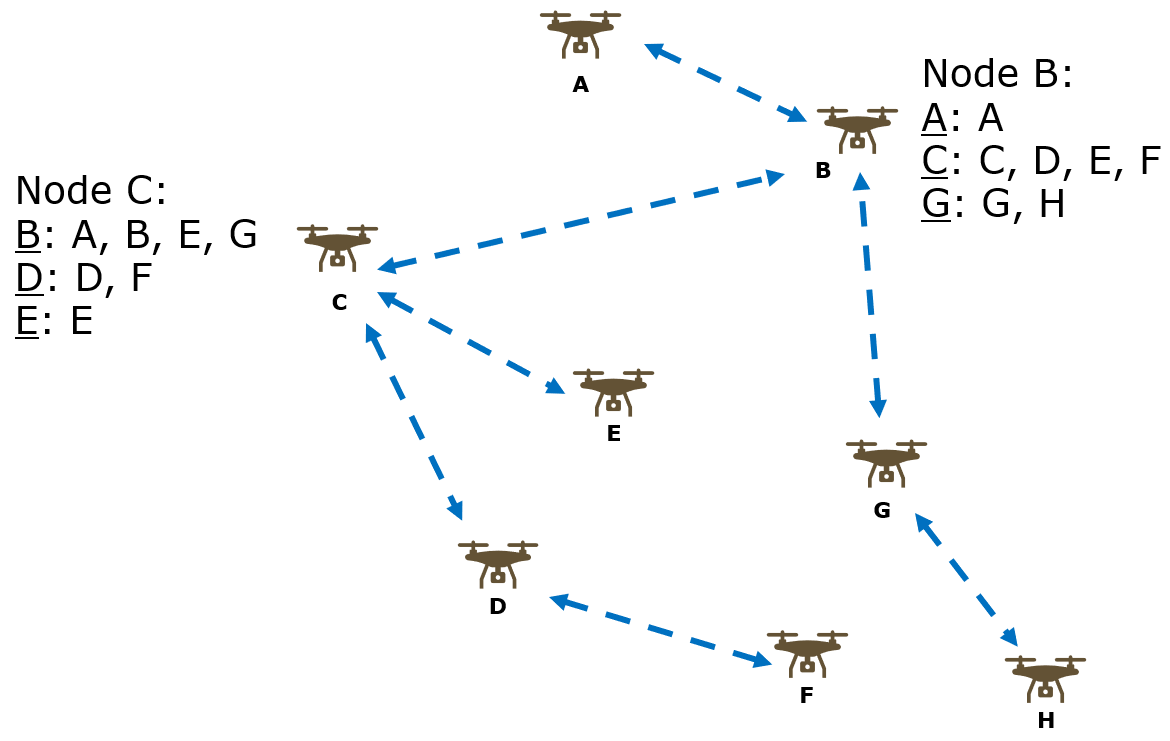
\includegraphics[width=\textwidth,keepaspectratio]{Images/Chpt2/BATMAN_topology.png}
    \caption{An overview of an individual EMANE emulated network node.}
    \label{batman_topology}
\end{figure}

\subsection{Reactive Routing}
    % Does not require maintenance and therefore generates less traffic
    % Topology updates are only discovered when a previously discovered route fails
The either primary category of MANET routing protocol are reactive protocols, also sometimes referred to as "on-demand" protocols~\cite{manet_survey}.
These protocols are referred to as on-demand protocols because routes to a destination are only found, when the transmitting node requires them.
This has the benefit of greatly reducing control traffic present in the network since topology and link state information is not periodically shared, but it does result in higher latency as traffic must wait for a route to be found.
This type of routing protocol could be beneficial in a network that is constrained on bandwidth and will typically only contain traffic that is not time-sensitive.\par
    % Examples:
        % AODV
        % DSR
Two examples of reactive MANET protocols are AODV and DSR~\cite{reactive_routing}.
These protocols generally act by sending out request packets upon needing a route, indicating the destination the traffic is intended for, and waiting for a response.
Nodes that have a route to that destination response, and once a full route is found the traffic is sent along it.
The route is then stored and considered a good route for that traffic until an attempt at using the route fails.
At that point the discovery process is repeated finding a new route.\par
    % BATMAN tends to have less available bandwidth than AODV, but more reliably delivers packets and detects topology changes faster
Generally, reactive protocols are found to not be as effective in highly mobile MANETs \cite{aodv_batman,reactive_routing}.
B.A.T.M.A.N. is found to have less maximum available bandwidth in some situations when compared to AODV, but will more reliably deliver packets successfully, and often is able to react to changes in the graph faster.
For this reason, proactive protocols like OLSR and B.A.T.M.A.N. are more commonly used in simple EMANE testbeds, as seen in the tutorial~\cite{emane_tutorial}.\par
All the testbeds in the remainder of this thesis will use the batman-adv implementation of the B.A.T.M.A.N. protocol.
This implementation is built into the Linux kernel and installation instructions for using it can be found in Appendix~\ref{appendixa}.

\section{Chapter Summary}
    % Chapter covered the basics of EMANE so that it may be used to set up and run experiments
    % Mobile ad-hoc routing is important to understand the operation of the robot swarm experiment
This chapter covered necessary background information on the differences between testing networks in hardware, testing networks in simulation, and testing networks in emulation.
Network hardware testbeds are expensive and so simulation or emulation were decided to be used instead.
Several network simulators including ns-3, OMNeT++, CORE, and EMANE were examined, and the emulator EMANE was determined to be the best tool for this thesis thanks to its accurate modeling of the PHY and MAC layers, mechanisms to individual control the software running on each node, and ability to interface with hardware.
Having selected EMANE, installation instructions were detailed, and an overview of the tool and its subsystems was presented.
The chapter then finished by presenting an overview of MANET routing protocols, the type of protocol that will be used in the EMANE testbeds detailed over the next three chapters.